% !TeX root = RJwrapper.tex
\title{tmap: An R Package for thematic maps}
\author{by Martijn Tennekes}

\maketitle

\abstract{
A thematic map is a geographical map in which statistical data are visualized. The theme refers to the statistical phenomena that is shown, such as the unemployment rate at municipal level. 
The best known thematic map type is the choropleth, where regions are coloured according to a statistical variable, for instance unemployment rate. Another popular thematic map type is the bubble map, in which the sizes of the bubbles are defined by a statistical variable, for instance metropolitan population.
With the \CRANpkg{tmap} package, thematic maps can be generated with great flexibility. A thematic map is created by stacking layers, for instance one for colouring municipalities, one for thick borders of higher level regions, and one for text labels. 
The standard work flow that is needed to create a thematic map is embedded in tmap by several convenient functions for reading, appending, and transforming spatial data.
}



\section{Introduction}
%Introductory section which may include references in parentheses \citep{R}, or cite a reference such as \citet{R} in the text.

Visualization is key in data science. Without looking at data, it is difficult to know the data, to unveil anomalies, and, moreover, to extract valuable knowledge~\citep{tufte83}. Software tools to visually explore, analayse, and present data should therefore belong to any data scientist's toolkit. The R language and its packages contain many functions to craft elegant and clarifying graphics, most notably \CRANpkg{ggplot2 }\citep{ggplot2}. Although it is also possible to achieve great looking geospatial visualizations, it is often more complicated and requires the usage of several R pacakges together. Therefore, I introduce the \CRANpkg{tmap} package by which thematic maps can be created in a flexible and layer-based way.

Thematic maps are geographic maps in which spatial data distributions are shown, such as population density. Although they are widely used for publication purposes, which is no surprise due to their visual appeal and recognizability, they also proved to be succesful for discovery and exploration of spatial data~\citep{friendly95}. One of the most illustrative examples is the dot map that physician John Show used to locate the source of the cholera outbreak in London in 1854~\citep{snow1855}. Roughly, there are five types of thematic maps:

\begin{description}
\item[choropleth] Administrative areas are colored according to a variable.
\item[proportional symbol map] Symbols are scaled in proportion to a variable. The best know variant is the bubble map.
\item[dot map] Individual data points are positioned on the map, like the cholera occurences in John Snow's map.
\item[isopleth] Regions are defined by homogeneity of a quantitative variable. For instance altitude or wheather maps.
\item[cartogram] The geographic maps is distorted. Regions are sized according to a quantitative variable.
\end{description}



The aim of the \CRANpkg{tmap} package is to provide R users an elegant and flexible way of making thematic maps, with a minimum of code required. The syntax resembles the syntax of \CRANpkg{ggplot2}, and follows the layered grammar of graphics~\citep{wickham10} broadly. All of the described thematic map types can be created with \CRANpkg{tmap} except the cartogram. 


Cartograms are not supported yet. Also, isopleths cannot be made in a straightforward manner with \CRANpkg{tmap}. Typically the \CRANpkg{raster}~\citep{raster} package provides excellent options for this.





%\section{A quick example}
%
%\begin{example}
%#load spatial objects contained in tmap
%data(Europe)
%data(metro)
%\end{example}

\section{An example}

A thematic map of the world that has been created with \CRANpkg{tmap} is depicted in Figure~\ref{figure:bubblemap}. It shows the relation between level of income per country and the distribution of emerging metropolitan areas. While the metropolitan areas in high income countries have a annual growth rate that is less than two percent (notice that the world population increases with 2.7 percent), metropolitan areas in lower income countries grow very fast, especially in Asia but also western and middle Africa.

\begin{widefigure}[htbp]
  \centering
  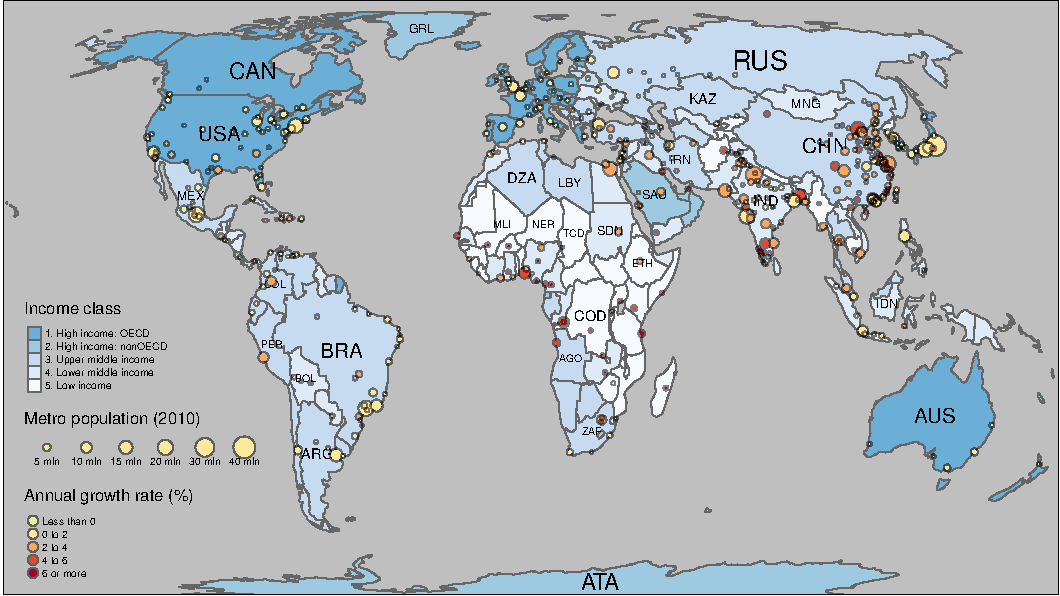
\includegraphics{bubbleMap2}
  \caption{World map about income and urbanization.}
  \label{figure:bubblemap}
\end{widefigure}

The code required to create this map is the following.

\begin{example}
#load spatial objects contained in tmap
data(World)
data(metro)

#derive new variable
metro$growth <- (metro$X2020 - metro$X2010) / (metro$X2010 * 10) * 100

#plot
tm_shape(World) +
  tm_fill("income_grp", style="kmeans", palette="-Blues") +
  tm_borders() +
  tm_text("iso_a3", size="AREA", scale=1.5) +
tm_shape(metro) +
  tm_bubbles("X2010", col = "growth", border.col = "black", 
    border.alpha = .5, style="fixed", breaks=c(-Inf, 0, 2, 4, 6, Inf) ,
    palette="-RdYlGn", contrast=1) + 
tm_layout_World(title="", legend.titles=c(fill="Income class", 
  bubble.size="Metro population (2010)", bubble.col="Annual growth rate (%)"))
\end{example}

The \code{\#plot} part of the code is exampled in detail in section~\ref{syntax}. In a nutshell, two groups of layers are drawn. The first group defines a choropleth that uses the \code{SpatialPolygonsDataFrame} object \code{World}. The drawing layers define the fill colors of polygons (\code{tm\_fill}), their borders (\code{tm\_borders}), and the supplementary text labels (\code{tm\_text}). The second group defines a bubble map based on the \code{SpatialPointsDataFrame} metro. The only layer consist of the bubbles created by \code{tm\_bubbles}.

%Notice the similarities with the \CRANpkg{ggplot2} syntax. 


\section{Related R-packages}



The \CRANpkg{tmap} package stands on the shoulders of the following six great packages.

\begin{description}
\item[\CRANpkg{sp}~\citep{sp1, sp2}] This package contains classes and methods for spatial data. %Only spatial objects from SpatialPolygons(DataFrame), SpatialPoints(DataFrame) and SpatialLines(DataFrame) are accepted.
\item[\CRANpkg{rgdal}~\citep{rgdal}] Reading and writing ESRI shape files is done by this package, as well as map projections via the PROJ.4 library~\citep{proj4}.
\item[\CRANpkg{rgeos}~\citep{rgeos}] All geometric processing is carried out by this package.
\item[\CRANpkg{classInt}~\citep{classInt}] This package facilitates class intervals, which are used in choropleths of quantitative variables.
\item[\CRANpkg{RColorBrewer}~\citep{classInt}] All used color schemes have been proposed by~\citet{brewer03} and implemented in this package.
\item[\CRANpkg{grid}] This package provides all basic plotting functions.
\end{description}







\section{Syntax}\label{syntax}


%This section may contain a figure such as Figure~\ref{figure:rlogo}.
%

\section{Another section}

There will likely be several sections, perhaps including code snippets, such as:


\section{Summary}

This file is only a basic article template. For full details of \emph{The R Journal} style and information on how to prepare your article for submission, see the \href{http://journal.r-project.org/latex/RJauthorguide.pdf}{Instructions for Authors}.


\address{Martijn Tennekes\\
  Statistics Netherlands\\
  CBS-Weg 11, 6412 EX Heerlen\\
  Netherlands\\}
\email{mtennekes@gmail.com}

\bibliography{tennekes}
